\documentclass[8.01x]{subfiles}
\begin{document}

\chapter{Week 14: Homework 10}

\section{Problem 1: Bar on rollers}

\begin{center}
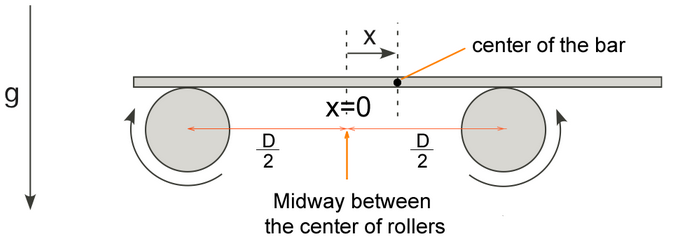
\includegraphics[scale=0.7]{Graphics/h10p1}
\end{center}

``A bar of mass $m$ and negligible height is lying horizontally across and perpendicular to a pair of counter rotating rollers as shown in the figure. The rollers are separated by a distance $D$. There is a coefficient of kinetic friction $\mu_k$ between each roller and the bar. Assume that the bar remains horizontal and never comes off the rollers, and that its speed is always less than the surface speed of the rollers. Take the acceleration due to gravity to be $g$.

(a) Find the normal forces $N_L$ and $N_R$ exerted by the left and right rollers on the bar when the center of the bar is displaced a distance $x$ from the position midway between the rollers. Express your answers in terms of $m$, $x$, $d$ and $g$.''

b) Find the differential equation governing the horizontal displacement of the bar $x(t)$. Express your answer in terms of $x$, $d$, $\mu_k$ and $g$.

c) The bar is released from rest at $x = x_0$ at $t = 0$. Find the subsequent location of the center of the bar, $x(t)$. Express your answer in terms of $x_0$, $d$, $\mu_k$, $t$ and $g$.''

The recommended reading gives us a not-so-small hint that this is a simple harmonic oscillation.\\
With the condition given, there will always be slipping, and therefore always kinetic friction. We know nothing about the speed of the rotation, but since the frictional force is given by $\mu_k N$, that shouldn't matter, as long as there is always slipping.

Newton's second law in the horizontal direction (with rightwards as positive) gives us

\begin{equation}
m a_x = \mu_k N_L - \mu_k N_R = \mu_k (N_L - N_R)
\end{equation}

Rewritten,

\begin{equation}
\ddot{x} = \frac{\mu_k}{m} (N_L - N_R)
\end{equation}

Vertically (with upwards as positive):

\begin{equation}
0 = N_L + N_R - m g
\end{equation}

Two equations, three unknowns. Now, if the center of the bar is at $x>0$, it's clear that $N_R > N_L$, and vice versa if $x < 0$. The above equations doesn't account for that. The net torque on the bar (about the center, say) must also be zero, or it won't remain horizontal. We can capture that as

\begin{equation}
0 = (x + D/2) N_L - (D/2 - x) N_R
\end{equation}

since gravity acting at the center of mass can cause no torque relative to the center of mass. It's unfortunate that we need to find $N_L$ and $N_R$ too, or there would certainly be less algebra involved.  We begin by finding $N_L$ and $N_R$; for that, we only need the last two equations. After that, we have one (differential) equation and one unknown left.

The vertical force equation easily gives us

\begin{equation}
N_L = m g - N_R
\end{equation}

Solving the torque equation for $N_R$ gives us

\begin{equation}
\frac{(x + D/2)}{(D/2 - x)} N_L =  N_R
\end{equation}

Substitute that back:

\begin{align}
N_L &= m g - \frac{(x + D/2)}{(D/2 - x)} N_L\\
N_L &\left(1 + \frac{(x + D/2)}{(D/2 - x)}\right) = m g\\
N_L &= \frac{m g}{1 + \frac{(x + D/2)}{(D/2 - x)}}\\
N_L &= \frac{m g(D - 2x)}{2D}
\end{align}

And, substitute that into the equation for $N_R$, below:

\begin{align}
N_R &= m g - N_L\\
N_R &= m g - \frac{m g(D - 2x)}{2D}
\end{align}

For part (b), we substitute this back into the $\ddot{x}$ equation:

\begin{align}
\ddot{x} &= \frac{mu_k}{m} \left(\frac{m g(D - 2x)}{2D} - m g + \frac{m g(D - 2x)}{2D}\right)\\
\ddot{x} &= \mu_k g \left(\frac{D}{D}  - \frac{2x}{D} - 1\right)\\
\ddot{x} &= - \frac{2 \mu_k g x}{D}
\end{align}

The sign changes in step 1, since we get a double negative on the fraction when calculating $N_L - N_R$. Finally, for part (c), we notice that this is a simple harmonic motion, and solve it accordingly.

\begin{align}
\ddot{x} + \mu_k g \frac{2}{D} x &= 0\\
x &= x_0 \cos(\omega t)\\
\omega &= \sqrt{\frac{2 \mu_k g}{D}}
\end{align}

So, all in all,

\begin{equation}
x = x_0 \cos\left(\sqrt{\frac{2 \mu_k g}{D}} t \right)
\end{equation}

If we write $x$ as $x = \cos (\omega t + \varphi)$ and set $t = 0$, we find

\begin{equation}
x_0 = x_0 \cos(\varphi)
\end{equation}

and so $\cos(\varphi) = 1 \Rightarrow \varphi = 0$, which is why I didn't include it above. (I figured as much since it was released from rest, not to mention they didn't ask for it.)

\section{Problem 2: Table problem: Rolling solution}

\begin{center}
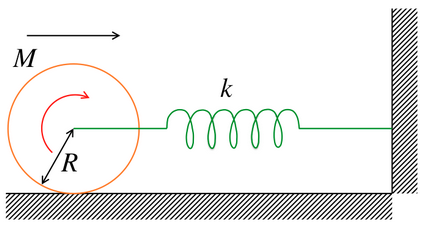
\includegraphics[scale=0.7]{Graphics/h10p2}
\end{center}

``Attach a solid cylinder of mass $M$ and radius $R$ to a horizontal massless spring with spring constant $k$ so that it can roll without slipping along a horizontal surface. If the system is released from rest at a position in which the spring is stretched by an amount $x_0$ what is the period $T$ of simple harmonic motion for the center of mass of the cylinder? Express your answer in terms of $M$ and $k$.''

First, let's identify the forces present. There's the spring force of magnitude $k x$, and the frictional force $F_f$.\\
When the spring is stretched, the spring force is towards the right, in the direction of the acceleration. The frictional force is opposite that, and will provide a torque that causes the cylinder to roll.\\
If we use rightwards as positive (since the acceleration will begin in that direction), $k x$ will begin negative, since the initial position is $x = -x_0$. As usual, then, we must write $- k x$ for the spring force. The frictional force also has a negative, since it's towards the left when the acceleration is positive:

\begin{equation}
m \ddot{x} = - k x - F_f
\end{equation}

Next, since there is pure roll, we can use $a = \ddot{x} = \alpha R$. We also have that $\tau = I \alpha$, which leads us to (via $\tau = R F_f$ and $\displaystyle I = \frac{1}{2} M R^2$):

\begin{align}
R F_f &= (\frac{1}{2} M R^2) (\ddot{x}/R)\\
F_f &= \frac{1}{2} M \ddot{x}
\end{align}

We could also write an equation relating vertical forces, but it turns out we don't need to.\\
If we substitute the value of $F_f$ into the previous equation,

\begin{align}
M \ddot{x} &= - k x - \frac{1}{2} M \ddot{x}\\
\frac{3}{2} M \ddot{x} &= - k x\\
\ddot{x} + \frac{2 k}{3 M} x &= 0
\end{align}

A simple harmonic oscillation, as we would expect. The solution is then

\begin{align}
x &= x_0 \cos(\omega t + \pi)\\
\omega &= \sqrt{\frac{2 k}{3 M}}\\
T &= \frac{2 \pi}{\omega} = 2 \pi \sqrt{\frac{3 M}{2 k}}
\end{align}

where I wrote the phase as $\pi$ since at $t = 0$, we need $x = -x_0$. I could also have written the entire right-hand side as negative.

\section{Problem 3: U-tube}

\begin{center}
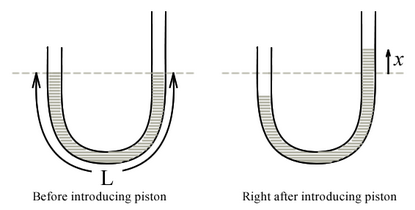
\includegraphics[scale=0.7]{Graphics/h10p3}
\end{center}

``A U-tube open at both ends to atmospheric pressure $P_0$ is filled with an incompressible fluid of density $\rho$. The cross-sectional area $A$ of the tube is uniform and the total length of the column of fluid is $L$. A piston is used to depress the height of the liquid column on one side by a distance $x_0$, and then is quickly removed. What is the frequency of the ensuing simple harmonic motion? Assume streamline flow and no drag at the walls of the U-tube. (Hint: use conservation of energy). Express your answer in terms of $L$ and acceleration due to gravity g.''

Hmm, we've done this in lecture already, but let's re-derive it, then.\
The liquid has a velocity that is the same everywhere (under these conditions), $\dot{x}$. Therefore, the liquid as a whole has a kinetic energy of

\begin{equation}
\frac{1}{2} M \dot{x}^2 = \frac{1}{2} A L \rho \dot{x}^2
\end{equation}

There is also gravitational potential energy. We define $U = 0$ at the equilibrium point. The change is then that a height of fluid $x$ of mass $m = A x \rho$ is moved upwards a distance $x$. (It's essentially taken from the left side and moved upwards on the right side, gaining potential energy.)\\
The sum of these two energies must be a constant:

\begin{equation}
\frac{1}{2} A L \rho \dot{x}^2 + A x \rho g x = \text{constant}
\end{equation}

using $m g h = (A x \rho) g x$.

We take the time derivative of this; the rate of change in the energy must be zero if it's constant, which the differentiation takes of for us.

\begin{align}
\frac{1}{2} A L \rho \dot{x}^2 + A \rho g x^2 &= \text{constant}\\
\frac{1}{2} A L \rho 2 \dot{x} \ddot{x} + A \rho g 2 x \dot{x} &= 0\\
L  \ddot{x} + 2 g x &= 0\\
\ddot{x} + \frac{2 g}{L} x &= 0
\end{align}

$\dot{x}$, $A$ and $\rho$ cancel, and we end up with a simple harmonic oscillation, as expected (and as usual, at this point!). The solution is

\begin{align}
x &= x_0 \cos(\omega t)\\
\omega &= \sqrt{\frac{2 g}{L}}\\
f &= \frac{1}{2\pi} \sqrt{\frac{2 g}{L}}
\end{align}

... though in reality there will be losses which cause damping, so $T$ will be longer, and the amplitude will decrease rather rapidly, rather than stay constant forever as this solution predicts.

\section{Problem 4: Liquid density}

\begin{center}
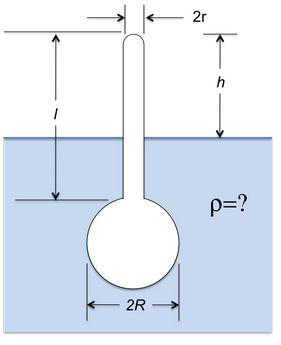
\includegraphics[scale=0.7]{Graphics/h10p4}
\end{center}

``A hydrometer is a device that measures the density of a liquid. The one shown in the figure has a spherical bulb of radius $R$ attached to a cylindrical stem of radius $r$ and length $\ell$. When placed in a liquid, the device floats as shown in the figure with a length $h$ of stem protruding. Given that the mass of the hydrometer is $M$, find the density $\rho$ of the liquid. Express your answer in terms of $M$ ,$R$, $r$, $\ell$ and $h$.''

The total volume of the hydrometer is

\begin{equation}
V_{sphere} + V_{cylinder} = \frac{4}{3} \pi R^3 + \pi r^2 \ell
\end{equation}

while the submerged part is

\begin{equation}
\frac{4}{3} \pi R^3 + \pi r^2 (\ell - h)
\end{equation}

Since it floats, the upwards buoyant force must be equal to the downwards gravitational force $M g$.\\
The buoyant force is equal to the weight of the displaced water, which is the submerged volume times $\rho$ (which is its mass) times $g$. That is,

\begin{equation}
M g = \rho g \left(\frac{4}{3} \pi R^3 + \pi r^2 (\ell - h)\right)
\end{equation}

\begin{equation}
\rho = \frac{M}{\frac{4}{3} \pi R^3 + \pi r^2 (\ell - h)}
\end{equation}

\section{Problem 5: Venturi flow meter}

\begin{center}
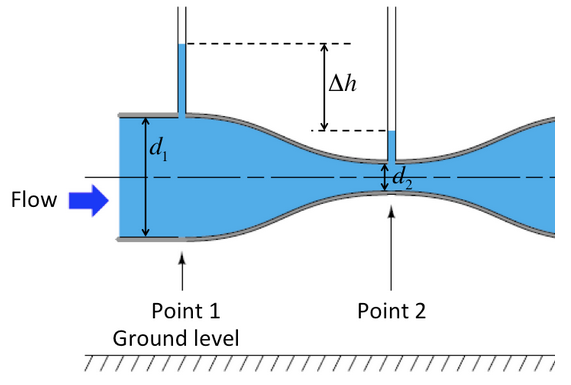
\includegraphics[scale=0.6]{Graphics/h10p5}
\end{center}

``A Venturi flow meter is used to measure the the flow velocity of a water main. The water main has a diameter of $d_1 = 40.0$ cm, and the constriction has a diameter of $d_2 = 20.0$ cm. The two vertical pipes are open at the top, and the difference in water level between them is $\Delta h = 2.0$ m. Find the velocity $v_m$ (in m/s), and the volumetric flow rate $Q$ (in $\text{m}^3/\text{s}$), of the water in the main.''

The volumetric flow rate must be the same both the thick part at $d_1$ and the thinner at $d_2$, since water is practically incompressible.\\
Therefore, the velocity must be greater at point 2 than at point 1.\\
I will, for consistency, use $v_1$ for the velocity at point 1; $v_1 = v_m$.

\begin{align}
Q &= v_1 A_1 = v_2 A_2\\
Q &= v_1 \pi \left(\frac{d_1}{2}\right)^2 = v_2 \pi \left(\frac{d_2}{2}\right)^2
\end{align}

This gives us

\begin{equation}
v_1 d_1^2 - v_2 d_2^2 = 0
\end{equation}

We can also relate the energies at the two points via Bernoulli's equation. We have kinetic energy (per unit volume), gravitational potential energy (per unit volume), and pressure. The GPE is equal at the two points, as they are at equal height with equal $\rho$, so if we wrote it down it would simply cancel.

\begin{equation}
\frac{1}{2} \rho v_1^2 + P_1 = \frac{1}{2} \rho v_2^2 + P_2
\end{equation}

We don't know $v_1$, $v_2$, $P_1$ or $P_2$, so we have four unknowns. We can rewrite this a bit, though.

\begin{equation}
P_1 - P_2 = \frac{1}{2} \rho \left(v_2^2 - v_1^2\right) \label{eq:h10p5_energy}
\end{equation}

We can use the height of the water columns to figure out the pressure difference.

The air at the top of the water columns are at atmospheric pressure, call it $P_0 = \SI{1}{atm}$.\\
The height of the left column, measured from the horizontal center line, depends on $P_1 - P_0$, via Pascal's law:

\begin{equation}
P_1 - P_0 = \rho g h_1
\end{equation}

The right column is similar.

\begin{equation}
P_2 - P_0 = \rho g h_2
\end{equation}

We don't know $h_1$ or $h_2$, but we know $h_1 - h_2= \Delta h$. If we subtract the two equations,

\begin{align}
(P_1 - P_0) - (P_2 - P_0) &= \rho g h_1 - \rho g h_2\\
P_1 - P_2 &= \rho g \Delta h
\end{align}

We use this in equation \eqref{eq:h10p5_energy}. That gives us these two equations (after $\rho$ cancels):

\begin{align}
g \Delta h &= \frac{1}{2} \left(v_2^2 - v_1^2\right)\\
v_1 d_1^2 - v_2 d_2^2 &= 0
\end{align}

Since we don't care about $v_2$, we can solve the second equation for it, substitute that into the first, and then just forget about $v_2$ altogether.

\begin{equation}
v_2 = v_1 \frac{d_1^2}{d_2^2}
\end{equation}

\begin{align}
2 g \Delta h &= \left(v_1 \frac{d_1^2}{d_2^2}\right)^2 - v_1^2\\
2 g \Delta h &= v_1^2 \left(\frac{d_1^4}{d_2^4} - 1\right)\\
\sqrt{\frac{2 g \Delta h}{\frac{d_1^4}{d_2^4} - 1}} &= v_1\\
\sqrt{\frac{2 g \Delta h\ d_2^4}{d_1^4 - d_2^4}} &= v_1
\end{align}

For the number we were given, this gives us $v_1 = v_m = \SI{1.6174}{m/s}$.\\
Using the simple relationship $\displaystyle Q = v_1 A_1  = v_1 \left(\frac{d_1}{2}\right)^2$ we find a flow rate of $Q = \SI{0.203}{m^3/s}$.

\section{Problem 6: Bucket with a hole}

\begin{center}
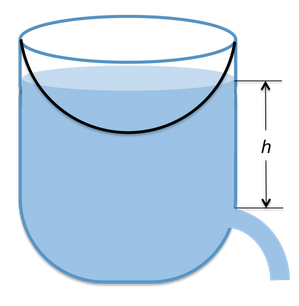
\includegraphics[scale=0.6]{Graphics/h10p6}
\end{center}

``A cylindrical bucket has a small hole at the bottom. The water exiting the hole has velocity $v$. What is the depth, $h$, of the water in the bucket?''

I suppose the question is rather ``at what depth $h$ is the hole located'', according to the picture.\\
Let's see, what facts do we have? Not a whole lot in terms of given facts, but if we add to that the things discussed in lecture (and in the book), we have a lot more.

We can solve this in multiple ways, I noticed.

\subsection{Solution 1}

The pressure at that depth is $P_1 = \SI{1}{atm} + \rho g h$. The pressure difference between inside and outside the bucket is then simply $\rho g h$.\\
We can apply Bernoulli's equation here, again while ignoring the term related to gravitational potential energy, as there is no height difference involved (if we consider a point at that depth, but at the container's left side, as being inside). Using $P_1$ for the pressure inside the bucket at depth $h$, and $P_2$ for the pressure outside:

\begin{align}
\frac{1}{2} \rho v_{inside}^2 + P_1 &= \frac{1}{2} \rho v^2 + P_2\\
\frac{1}{2} \rho v_{inside}^2 + \SI{1}{atm} + \rho g h &= \frac{1}{2} \rho v^2 + \SI{1}{atm}\\
\frac{1}{2} v_{inside}^2 + g h &= \frac{1}{2} v^2\\
h &= \frac{v^2}{2g}
\end{align}

Here, I consider $v_{inside}$ to be negligible compared to $v$, so I ignore it. It we consider $v_{inside}$ to be the velocity \emph{just} inside the hole, that is clearly not correct. However, the rest of the equation is equally valid at the leftmost edge of the container.

\subsection{Solution 2}

I feel a bit funny about the assumption $v_{inside} = 0$ while considering a point at depth $h$ in the liquid, as the equation doesn't specify where that point is: near the hole, or far from it.\\
We can solve this in a slightly different way. We again begin with Bernoulli's equation, but this time, we consider a point at the surface of the liquid (above the hole), and a point just outside the hole. Both are exposed to the atmosphere, so $P_1 = P_2 = \SI{1}{atm}$ and we don't need to specify that in the equation, as it will simply cancel.

Instead, we have the gravitational potential energy per unit volume, $\rho g y$, in the equation. On the left side, we have at the top of the container, where it is $\rho g h$; I define the zero level to be at the hole, so the term only exists on the left-hand side.

\begin{align}
\frac{1}{2} \rho v_{surface}^2 + \rho g h &= \frac{1}{2} \rho v^2\\
2 g h &= v^2\\
h &= \frac{v^2}{2 g}
\end{align}

As before, we approximate the other velocity, this time at the surface, to be zero. We find exactly the same result using this method.

\section{Problem 7: Buoyant force of a balloon}

``Helium balloons are used regularly in scientific research. A typical balloon would reach an altitude of 40.0 km with an air density of $\SI{4.3e-3}{kg/m^3}$. At this altitude the helium in the balloon would expand to $\SI{540000.0}{m^3}$. Take $g = \SI{10}{m/s^2}$. Find the buoyant force on the balloon.''

The buoyant force is given by the weight of the displaced fluid -- air in this case -- so this should be very simple. Weight is given by mass times $g$, while mass is $\rho V$, so $F_B = V \rho_{air} g$:

\begin{equation}
F_B = (\SI{540000.0}{m^3})(\SI{4.3e-3}{kg/m^3})(\SI{10}{m/s^2}) \approx 23220 N
\end{equation}

Very simple indeed.

\end{document}
